%# -*- coding: utf-8-unix -*-
%%==================================================
\chapter{C++}
\label{chap1}
\begin{itemize}[noitemsep,topsep=0pt,parsep=0pt,partopsep=0pt]
	\item ...
\end{itemize}

\section{知识点和方法论}
\subsubsection{map 和 unordered\_map 不同点}

map 内部实现了一颗红黑树, 红黑树有自动排序的功能.

unordered\_map 内部实现了一个哈希表, 如果遇到冲突, 同位置上的元素节点小于8个的时候, 这些数据会是一个链表式的方式互相连起来。 当同位置上的元素节点大于8个的时候, 会自动转化为成一个map(红黑树)。

\subsubsection{C++ 不能重载的运算符}
$$. :: .* ?: sizeof$$

大多数运算符都是可以重载的,但是有5个运算符C++语言规定是不可以重载的.

1. .(点运算符),通常用于去对象的成员,但是->(箭头运算符),是可以重载的

2.::(域运算符),即类名+域运算符,取成员,不可以重载

3..*(点星运算符,)不可以重载,成员指针运算符".*,即成员是指针类型

4.?:(条件运算符),不可以重载

5.sizeof,不可以重载
\subsubsection{C++ 如果一个类中没有任何属性,占用空间为1, 这是规定}

不是规定哦, 为了确保两个不同对象的地址不同, 必须如此, 类的实例化是在内存中分配一块地址, 同样空类也会日次, 所以编译器会给空类隐含的添加一个字节, 这样空类是细化后就有独一无二的地址了. 所以, 空类的sizeof为1, 而不是0.

\subsubsection{返回引用}

优点:

1. 防止返回对象的时候调用拷贝构造函数和析构函数导致不必要的开销, 降低赋值运算符等的效率

2. 允许进行连续赋值

\subsubsection{类和结构体的区别}

默认继承访问权限区别, 类默认是private, struct 默认是 public.

简单来说, 抽象思维来判定是否要使用struct 或者是class, struct 是数据结构, class 是对象.

class 可以用来定义模板参数, struct 不可以

\subsubsection{类的大小}

\begin{lstlisting}
class A{};
class B{
	virtual void f(){};
};
class C: public B{};
class D: public virtual A{ // 虚继承 防止 菱形继承造成奇异
};

int main() {
	cout << sizeof(A) << endl;//1
	cout << sizeof(B) << endl;//8
	cout << sizeof(C) << endl;//8  虚函数表的地址 因为是64位系统所以sizeof是8
	cout << sizeof(D) << endl;//8  因为包含指向虚基类的指针
}
\end{lstlisting}


\subsubsection{C++ 内存对齐}
简单来说就是, 默认是4字节对齐. 对于一个结构体而言, 里面的顺序会对对齐字节产生影响. 参考链接
\url{https://zhuanlan.zhihu.com/p/30007037}

\subsubsection{C++11}
auto 类型推到
$$
	auto a = 10;
$$

众所周知C++11新增了右值引用,这里涉及到很多概念:

左值:可以取地址并且有名字的东西就是左值。

右值:不能取地址的没有名字的东西就是右值。

纯右值:运算表达式产生的临时变量、不和对象关联的原始字面量、非引用返回的临时变量、lambda表达式等都是纯右值。

返回值优化:当函数需要返回一个对象实例时候,就会创建一个临时对象并通过复制构造函数将目标对象复制到临时对象,这里有复制构造函数和析构函数会被多余的调用到,有代价,而通过返回值优化,C++标准允许省略调用这些复制构造函数。

\textbf{std::function \& std::bind \& lambda表达式}

\textbf{std::thread 线程相关 智能指针}


\textbf{委托构造函数}

\textbf{继承构造函数 using Base::Base}

\textbf{nullptr}

\textbf{final \& override}

\textbf{default and delete}

\textbf{explicit} 只能显示构造不能隐式转换.

\textbf{修饰类成员函数,表示在该函数内不可以修改该类的成员变量。 const } 比如  void func() const;

\textbf{constexpr } 运行期间就会被运算出来就是常量, 否则是普通函数.

\textbf{minmax\_element:返回容器内最大元素和最小元素位置}

\url{https://zhuanlan.zhihu.com/p/139515439}

\subsubsection{C++14特性}

auto 返回值推导

支持变量模板

[[deprecated]] 警告标记

\subsubsection{C++17特性}

C++17正式将file\_system纳入标准中,提供了关于文件的大多数功能,基本上应有尽有

\subsubsection{C++20特性}

auto res = foo <=> bar;

import 和 export

\subsubsection{模板类的函数定义}
\begin{lstlisting}
template <typename T>
void vector<T>::clear() {
	
}
\end{lstlisting}
\subsubsection{尾递归的实现}
简单来说, 如果直接返回结果的话会造成多次调用, 但是把返回的结果放在参数中, 编译器会进行一定的优化, 将其转为非递归的形式. 然后我们就可以减少爆栈的风险.

尾递归由于直接返回值,不需要保存临时变量,所以性能不会产生线性增加。并且编译器会将尾递归形式优化成非递归形式。


\subsubsection{socket 如何实现可靠连接}
1. 心跳包机制, 保持连接

2. 可以在正式数据发送前发送监测包, 刻骨短收到检测包后立即发挥一个响应. 服务端收到响应, 认为客户端还活着, 把正式数据发送


\subsubsection{set, multiset, map, multiset}
底层数据结构 使用红黑树, map/multimap使用pair作为基础元素. set/multiset value和key相同 \par
底层红黑树multi/nonulti 使用 insert\_unique 和 insert\_equal之间的差别 \par
\subsubsection{定义的静态全局变量作用于是}
本文件
\subsubsection{如何判断一段程序是由C编译器编译还是由C++编译器编译的}
有内置宏 \_\_cplusplus 是C++编译的
\subsubsection{在C++程序中调用被C编译器编译后的函数, 为什么要加extern"C"}
extern "C" 是修饰的变量和函数是按照C语言方式编译和链接的, 因为C编译器和C++编译器对一个函数的编译后的函数名是不同的, 这样为了实现混合查找函数名在类库中的实现,解决名字匹配问题. \par

\subsubsection{C++, const规则}
const只对它左边的东西起作用 ,  唯一的例外就是const本身就是最左边的修饰符,那么它才会对右边的东西起作用。 根据这个规则来判断就很容易了
\subsubsection{C++, const 和 \#define 之间的区别}
const和\#define 都能定义常量, 但是\#define只做单纯的替换, 但是const能进行代码安全检查.
\subsubsection{指针和引用之间的区别}
1. 指针可以指向空值 但是引用不能指向空值. \par
2. 指针可以不初始化, 引用必须初始化. \par
3. 指针可以随时更改指向的目标, 而引用初始化后就不可以再指向任何其他对象 \par
4. 指针可以进行地址偏移, 引用不可以 \par
\subsubsection{inline的优劣}
简单来说, 减少了函数调用, 但是增大了生成可执行程序的体积 \par
\subsubsection{C++11有什么你使用到的新特性}
auto 遍历的时候很方便 对于一些很复杂的变量直接使用auto, 让编译器去推断他的类型\par
lambda 表达式, 比如在sort中 可以很方便的写出cmp函数 \par
\subsubsection{C++中有malloc/free, 为什么还需要new/delete}
malloc/free是C/C++标准可以函数, new/delete是C++运算法. 他们都可以用于申请和释放内存. \par
对于类类型的对象而言, malloc/free 无法满足要求, 不会自动执行构造和析构函数. 因为C++需要new/delete \par
\subsubsection{面向对象技术的基本概念是什么,三个基本特征是什么?}
基本概念: 类、对象、继承; 基本特征: 封装、继承、多态。\par
\subsubsection{为什么基类的析构函数是虚函数?}
当我们使用基类的指针管理派生类,使用delete释放该指针时,会调用基类的析构函数~Base(),如果基类的析构函数是虚函数,那么就会继续调用派生类的析构函数~Derived();而如果基类的析构函数不是虚函数,就只会调用基类的析构函数,那么派生类中的那片内存就不会被释放,从而造成内存泄漏。 \par
\subsubsection{为什么构造函数不能为虚函数?}
答:虚函数采用一种虚调用的方法。需调用是一种可以在只有部分信息的情况下工作的机制。如果创建一个对象,则需要知道对象的准确类型,因此构造函数不能为虚函数。 \par

\subsubsection{如果虚函数是有效的,那为什么不把所有函数设为虚函数?}
答:不行。首先,虚函数是有代价的,由于每个虚函数的对象都要维护一个虚函数表,因此在使用虚函数的时候都会产生一定的系统开销,这是没有必要的。
\subsubsection{什么是多态?多态有什么作用?}
答:多态就是将基类类型的指针或者引用指向派生类型的对象。多态通过虚函数机制实现。
多态的作用是接口重用。
\subsubsection{重载和覆盖有什么区别?}
答:虚函数是基类希望派生类重新定义的函数,派生类重新定义基类虚函数的做法叫做覆盖;\par
重载就在允许在相同作用域中存在多个同名的函数,这些函数的参数表不同。重载的概念不属于面向对象编程,编译器根据函数不同的形参表对同名函数的名称做修饰,然后这些同名函数就成了不同的函数。
重载的确定是在编译时确定,是静态的;虚函数则是在运行时动态确定。
\subsubsection{什么是虚指针?}
答:虚指针或虚函数指针是虚函数的实现细节。带有虚函数的每一个对象都有一个虚指针指向该类的虚函数表。
\subsubsection{main函数执行之前会执行什么?执行之后还能执行代码吗?}
1. 全局对象的构造函数会在main函数之前执行 \par
2. 可以,可以用atexit注册一个函数(函数参数是一个函数指针),它会在main 之后执行; \par
\subsubsection{经常要操作的内存分为那几个类别?}
(1) 栈区:由编译器自动分配和释放,存放函数的参数值、局部变量的值等; 向下增长它的生长方式是向下的,是向着内存地址减小的方向增长。

(2) 堆:一般由程序员分配和释放,存放动态分配的变量;向上增长也就是向着内存地址增加的方向;

(3) 全局区(静态区):全局变量和(全局或局部)静态变量存放在这一块,初始化的和未初始化的分开放(.data 存放初始化后的数据  .bss 存放未初始化的数据);

(4) 常量区:常量字符串就放在这里,程序结束自动释放(.text 分区);

(5) 程序代码区:参访函数体的二进制代码。


//===============================另一本书书写

1. 栈: 在函数调用时存储参数, 返回地址和局部变量

2. 内存映射区: 文件到内存的映射和程序运行是申请的较大数据

3. 堆: 存储程序运行是申请的较小数据, 动态分配和销毁

4. BSS段: 存储未被初始化的全局变量和静态变量, 长度固定

5. 数据段: 存储已被初始化的全局变量和静态变量, 长度固定

6. 代码段: 存储程序的二进制代码, 长度固定

\subsubsection{链接器}
linux 中 g++ -o 将多个.o文件链接成一个可执行文件.

简单的来说, 我们针对一个.cc文件进行编译, 当做函数申明是存在的, 链接就是将这些函数找到. 链接也分为动态库链接.so, 和静态库链接 .a. 静态库链接直接打包的可执行文件中. 动态链接是, 不打包到文件中. 我们每次要用到动态库里面函数. 操作系统会帮我们找到动态库在哪里.

\subsubsection{符号表的作用}
编译器会生成一个叫做“符号表”的数据结构来维护变量名和内存地址直接的对应关系。它会搜集变量名,比如我们定义了一个全局的 int a; 那么编译器会为程序预留4个字节(32位平台)的空间,比如起始地址23456788(长度为4),并把变量名“a”和地址88888888保存进符号表,这样程序中对a进行相关操作时,它就会根据符号表找到变量的真正的物理位置(23456788),进行相关操作。 在机器执行程序的时候,会把变量名替换为内存地址(和长度),而不存在任何名称。


\subsubsection{函数指针与指针函数}
指针函数: 是函数, 但是返回指针(有两个括号) \par
函数指针: 是指针, 指向函数, 有四个括号 \par
\subsubsection{内部连接和外部链接有什么区别?}
1. 如果变量是内部链接的话, 那么此变量只能在当前文件内访问 \par
2. 如果变量是外部链接的话, 那么此变量可以被其他文件使用 \par
---\par
静态全局变量默认是内部链接, 而extern默认是外部链接 \par
\subsubsection{声明与定义的区别}
声明, 表示告诉编译器这个符号是存在的, 你先让我编译通过, 让连接器去找这个符号在哪里 \par
对于变量来说, 定义就是声明, 对于函数来说是有区别的, 如果没有实现函数体, 那么就是声明, 表示有这么一个函数. 至于函数在哪里.
\subsubsection{编译链接过程}
1. 预编译, 将\#include 和 \#define 展开, 生成.i文件 \par
2. 编译, 进行词法分析, 语法分析, 语义分析, 中间代码生成, 目标代码生成, 优化, 生成.s文件 \par
3. 汇编, 生成.o文件, 将汇编码翻译成机器码 \par
4. 链接, 地址和空间分配, 生成 .out 文件 \par
\subsubsection{C++函数中值的传递方式有哪几种?}
三种传递方式为:值传递、指针传递和引用传递。
\subsubsection{信号量和互斥量}
在C++中互斥量是mutex, 当一个线程获得了锁, 之后其他线程就不能访问到这个资源, 线程阻塞. 直到获得资源的线程unlock \par
在C++中叫做Semaphore, 信号量可以有多个, 如果值大于0, 则获得, 值减1, 如果值等于0, 则线程进入睡眠状态直到信号量大于0. \par
锁是服务于共享资源的; 而semaphore是服务于多个线程间多个资源的执行的逻辑顺序的。\par
\subsubsection{RVO和NRVO}
RVO(return value optimization ) 返回值优化, 防止产生临时对象. \par
\begin{lstlisting}
	Point3d factory()
	{
		Point3d x;
		return x;
	}
	Point3d p = factory();
\end{lstlisting}
优化成
\begin{lstlisting}
	Point3d p;
	factory(p);
	factory(const Point3d &_result)
	{
		Point3d x;
		result.Point3d::Point3d(x);  //复制构造函数 还没有吧x这个名字优化掉
		return;
	}
\end{lstlisting}
NRVO(name return value optimization) NRVO的优化比RVO 的优化更进一步,直接将要初始化的对象替代掉返回的局部对象进行操作。可以看出,进行NRVO 的优化后,此时整个函数将会只调用一次构造函数。
\begin{lstlisting}
	Point3d p;
	factory(p);
	factory(const Point3d &_result)
	{
		result.Point3d::Point3d(x); // 直接操作参数, 没有了x
		return;
	}
\end{lstlisting}
\subsubsection{听说过mangling么?}
简单来说, 就是C++为了函数重载实现的名称修改, 有一定的规则, 比如\_Z4funii \par
\subsubsection{模板代码如何组织?模板的编译以及实例化过程?}
模板类的声明要全部放在头文件中.
\subsubsection{C++中四种Cast的使用场景}
static\_cast<xxx>() : 表示编译级别的强制类型转换, 且不能发现运行是的错误. 类似C的(int) 之类的强制转圈, 不能去除const属性, volatile 属性. 还有一个unaligned属性 \par
dynamic\_cast<>() : 运行时检查类型. 主要用于含有虚函数的父类和子类之间的指针转换. 会检查是否能够完成这次转换, 如果不能返回0 \par
const\_cast<>(): 作为static\_cast的补充, 可以去除const属性 \par
reinterpret\_cast<>(): 低层次的类型转换, 可以将指针转为int类型或者long类型. \par
\subsubsection{C++什么是常量折叠}
简单来说, 我定义了一个const int 变量, 然后我对这个变量进行了修改, (用类型转化啥的) 然后, 输出值的时候还是原来的值, 因为输出的时候, 直接替换为了常量值. 其实值是被修改了的.
\subsubsection{为什么const修饰成员函数后不能修改成员变量}
每个成员函数在调用的时候,都会把this作为第一个参数传进去。我们在用const修饰成员函数的时候,就相当于修饰了this,也就是说我们的第一个参数应该是 const 类型 * this;
\subsubsection{auto\_ptr 被弃用了}
因为可能导致对同一块堆空间多次delete \par
\subsubsection{const int*}
const int * a1 = \&b; // 相当于 *a1 是固定的, a1是可变的 \par
int *const a2 = \&b; // 相当于 a2 是固定的, *a2是可变的

int const *a3 = \&b; // 等价于第一个 a1
\subsubsection{C++智能指针}
为什么要使用智能指针?

因为当传递过来一个指针对象, 我们不知道, 是否要进行资源的释放.
std::unique\_ptr  - 只有一个能拥有这个资源

Std::shared\_ptr -  很多个人能拥有这个资源但是这个资源的最后持有者会进行资源的释放操作.

Std::weak\_ptr - 简单来说是为了解决shared\_ptr循环引用造成资源泄露的问题.
\subsubsection{C++与java的不同点}
C++基于RTTI的机制进行运行时类型识别, 简单的说就是typeid + 四个cast进行类型的判断. 简单来说, typeid如果对于静态变量是静态编译的时候就可以做类型判定, 但是对于动态变量, 要运行是判定, 会造成一定的影响.
\begin{lstlisting}
class A{
	public:
	virtual void print() {
		cout << "I'm A\n"; 
	} 
};
class B : public A {
	public:
	void print() {
		cout << "I'm B\n";
	}
};

class C : public A {
	public:
	void print() {
		cout << "I'm C\n";
	}
};

int main () {
	A *p = new B();
	p->print();
	cout << typeid(p).name() << endl;
	if(typeid(p) == typeid(B*)) {
		cout << "p point b\n";
	}else if(typeid(p) == typeid(C*)) {
		cout << "p point c\n";
	}else if(typeid(p) == typeid(A*)) {
		cout << "p== \n";
	}
	//C * pc = dynamic\_cast<C*>(p); 
	// cat't succ
	// if(pc){
		//     pc->print();
		// }
	B * pb = dynamic\_cast<B*>(p);
	if(pb){
		pb->print();
	}
	const int a = 10;
	cout << typeid(\&a).name() << endl; //const int *
	cout << typeid(a).name() << endl; //const int *
	return 0;
\}
\end{lstlisting}

java 也有RTTI, 使用 instanceof , 或许加上反射(反射是大部分操作)
\begin{lstlisting}
class Base {}
class Derived extends Base {}

public class demo {
	public static void main(String[] args) {
		Derived derived = new Derived();
		System.out.println(derived instanceof Base); // 输出true
	}
}
\end{lstlisting}

\begin{lstlisting}
class Customer {
	private Long id;
	private String name;
	private int age;
	
	public Customer() {}
	
	public Customer(String name,int age) {
		this.name = name;
		this.age = age;
	}
	
	public Long getId() {
		return id;
	}
	public void setId(Long id) {
		this.id=id;
	}
	public String getName() {
		return name;
	}
	public void setName(String name) {
		this.name=name;
	}
	public int getAge() {
		return age;
	}
	public void setAge(int age) {
		this.age=age;
	}
	
}

class ReflectTester {
	public Object copy(Object object) throws Exception{
		// 获取对象类型
		Class classType=object.getClass();
		System.out.println("Class:" + classType.getName());
		
		// 通过默认构造方法创建一个新的对象
		Object objectCopy = classType.getConstructor(new Class[]{}).newInstance(new Object[]{});
		
		// 获取对象的所有属性
		Field fields[]=classType.getDeclaredFields();
		
		for(int i=0; i<fields.length; i++){
			Field field=fields[i];
			String fieldName=field.getName();
			String firstLetter=fieldName.substring(0,1).toUpperCase();
			System.out.println("firstLetter "+firstLetter);
			//获得和属性对应的getXXX()方法的名字
			String getMethodName="get"+firstLetter+fieldName.substring(1);
			// 获得和属性对应的setXXX()方法的名字
			String setMethodName="set"+firstLetter+fieldName.substring(1);
			
			// 获得和属性对应的getXXX()方法
			Method getMethod=classType.getMethod(getMethodName, new Class[]{});
			// 获得和属性对应的setXXX()方法
			Method setMethod=classType.getMethod(setMethodName, new Class[]{field.getType()});
			System.out.println("field.getType() " + field.getType());
			// 调用原对象的getXXX()方法
			Object value=getMethod.invoke(object, new Object[]{});
			System.out.println(fieldName+":"+value);
			// 调用拷贝对象的setXXX()方法
			setMethod.invoke(objectCopy, new Object[]{value});
		}
		return objectCopy;
	}
}
\end{lstlisting}
\subsubsection{C++异常和java异常处理的对比}
C++ 没有 finally, 因为c++中有一个非常重要的原则,就是:在异常发生前成功调用构造函数的类一定能够执行析构函数。

\begin{figure}
	\centering
	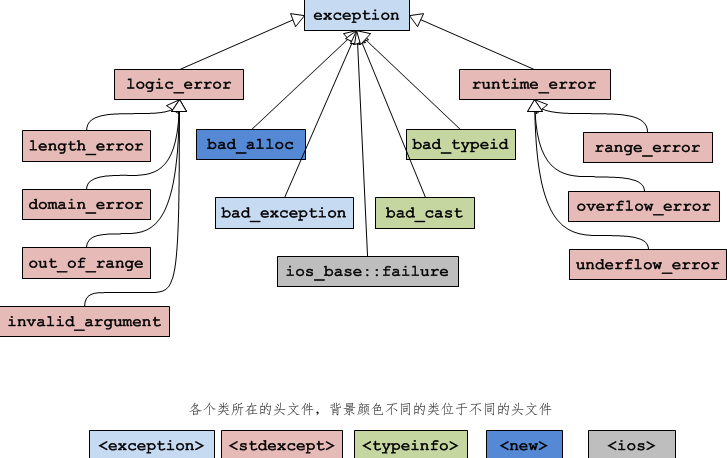
\includegraphics[width=0.7\linewidth]{figures/exceptioncpp.png}
	\caption{exception\_cpp}
	\label{fig:exception_cpp}
\end{figure}
但是不能捕获除0异常, 需要通过信号来实现 \url{http://blog.bitfoc.us/p/100}

java 继承于error 和  exception , exception 的异常能够捕获.

throw用在方法内,用来抛出一个异常对象,将这个异常对象传递到调用者处,并结 束当前方法的执行。

使用的格式:

throw new 异常类名(参数);


(throws)运用于方法声明之上,用于表示当前方法不处理异常,而是提醒该方法的调用者来处理异常

使用格式:

修饰符 返回值类型 方法名(参数) throws 异常类名1,异常类名2 ... { }
\begin{figure}
	\centering
	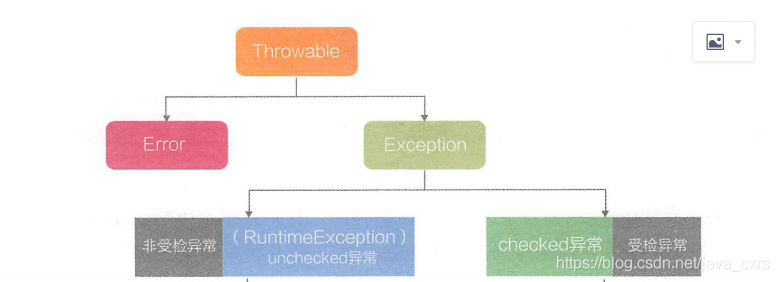
\includegraphics[width=0.7\linewidth]{figures/exceptionjava.png}
	\caption{exception\_java}
	\label{fig:exception_java}
\end{figure}


\subsubsection{C++虚函数原理}
1. 简单来说, 每一个含有虚函数的类都至少有一个与之对应的虚函数表, 其中存放着该类所有的虚函数对应的函数指针 \par
2. 在运行时, 会根据调用的指针指向的对象得到真正应该调用的函数, 然后通过偏移量找到虚函数地址并调用 \par
\subsubsection{C++虚函数表的开销}
1. 空间开销, 每个对象都会保持一个虚函数表造成空间开销 \par
2. 时间开销, 可能因为函数数简介寻址, 造成CPU分支预测失败造成流水线重刷性能开销 \par
\subsubsection{epoll水平触发\&epoll边缘触发}
对于监听的sockfd,最好使用水平触发模式,边缘触发模式会导致高并发情况下,有的客户端会连接不上。如果非要使用边缘触发,网上有的方案是用while来循环accept()。 \par
LT模式 \par
fd可读之后,如果服务程序读走一部分就结束此次读取,LT模式下该文件描述符仍然可读\par
fd可写之后,如果服务程序写了一部分就结束此次写入,LT模式下该文件描述符也仍然可写\par
ET模式 \par
fd可读之后,如果服务程序读走一部分就结束此次读取,ET模式下该文件描述符是不可读,需要等到下次有数据到达时才可变为可读,所有我们要保证循环读取数据,以确保把所有数据读出 \par
fd可写之后,如果服务程序写了一部分就结束此次写入,ET模式下该文件描述符是不可写的,我们要保证写入数据,确保把数据写满 \par
\subsubsection{传统IO和mmap}
1. 调用write, 告诉内核需要写入数据的开始地址与长度 \par
2. 内核将数据拷贝到内核页缓存 \par
3. 有操作系统调用, 将数据拷贝到磁盘, 完成写入. \par
Linux通过将一个虚拟内存区域与一个磁盘上的对象关联起来, 以初始化这个虚拟内存区域的内容. \par
可以减少一次拷贝.

\subsubsection{write 和 fwrite}
如果文件的大小是8k。
若用write,且只分配了2k的缓存,则要将此文件读入需要做4次系统调用。(内核空间和用户空间切换4次)
若用fwrite,则系统自动分配缓存,则读入此文件只要一次系统调用。
也就是用write要读4次磁盘,而用fwrite则只要读1次磁盘。所以fwrite的效率比write要高4倍。